\documentclass[12pt]{article}
\usepackage{sydewkrpt}
\usepackage{amsmath}

%%%%%%%%%%%%%%%%%%%%%%%%%%%%
%%%    Begin Document    %%%
%%%%%%%%%%%%%%%%%%%%%%%%%%%%
\begin{document}
\pagenumbering{roman}

\waterlootitle{ME 597: Assignment 2}{

  }{
  Sarah Elliott 20337924\\
  Leigh Pauls 20339616\\
  \today
  }

\newpage
\singlespacing
\pagenumbering{arabic}
\section{Inverse Measurement Model}
\setlength{\parindent}{1cm}

We simulated the IR range sensor array by taking the current position and orientation of the robot, the position and direction offsets of all 6 sensors, and the true ``ground map''. We then return 6 directed line segments. Each of those line segments represents the open space detected by a sensor.

The inverse measurement model first looks at the length of a returned line segment. If the line segment’s length is equal to the maximum range of the sensor, then it assumes that the sensor did not reflect off of any wall, and it is considered a ``clear'' line segment. If the line segment is less than the maximum, than it assumes that there is an obstacle at the end of the line segment, and it is considered a ``contacting'' line segment.

To update the probability map, the inverse measurement model iterates through each cell in the map. For each cell, it tests against each clear and contacting sensor line segment.
For each clear line segment, a ``pie slice'' is defined, with the pointy end at the start of the segment, and the center of the curved end at the end of the line segment. The width of the slice is defined by a constant Beta (10 degrees). If any of the current cell's corners, or its center point are within this pie slice, then the cell is updated to be considered ``clear''.
Each contacting line segment uses a similar update, but it instead uses 2 pie slices, a slightly longer ``contact'' pie slice, and a slightly shorter ``clear'' pie slice. The difference in size of the slices is defined by Alpha (0.1 meters). If any of the same points of the cell are within both slices, then the cell is considered clear, but if any are only in the contact slice, then the cell is considered occupied.
Each time that a cell is considered to be occupied or not, the update is performed by adding logit(0.7) or logit(0.4), respectively, to that cell's current logit ratio.


\newpage
\singlespacing
\section{Inverse Measurement Model Simulation}
\setlength{\parindent}{1cm}

\begin{figure}[ht]
\hspace{0.5cm}
\centering
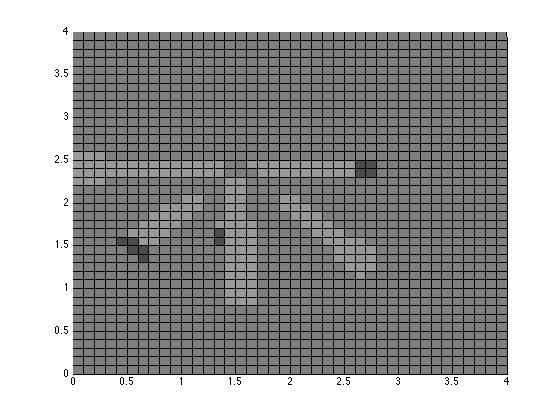
\includegraphics[scale=0.5]{Pictures/question2.png}
\caption{Single Map Update}
\end{figure}

This is a single update to the map given measurement lengths of [1, 1.5, 1.5, 0.8, 1.2, 1.5] from the robot’s left to right, for a robot positioned at [1.5, 2.5, 270 degrees].

\newpage
\singlespacing
\section{Exploration and Mapping}
\setlength{\parindent}{1cm}

We used a simple list of points to drive to to create an initial mapping of the environment, using logic of ``turn to the point, then drive straight''.

\begin{figure}[ht]
\hspace{0.5cm}
\centering
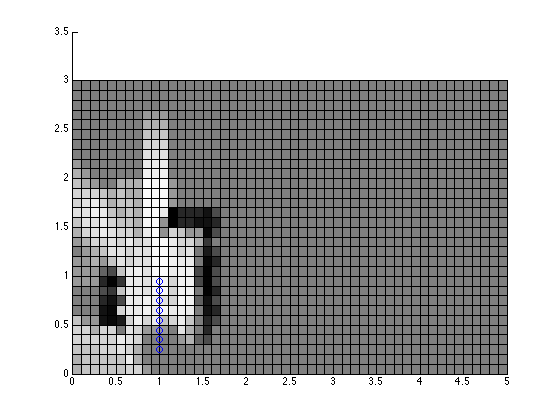
\includegraphics[scale=0.5]{Pictures/question3_15.png}
\caption{Map after 15 seconds}
\end{figure}

\begin{figure}[ht]
\hspace{0.5cm}
\centering
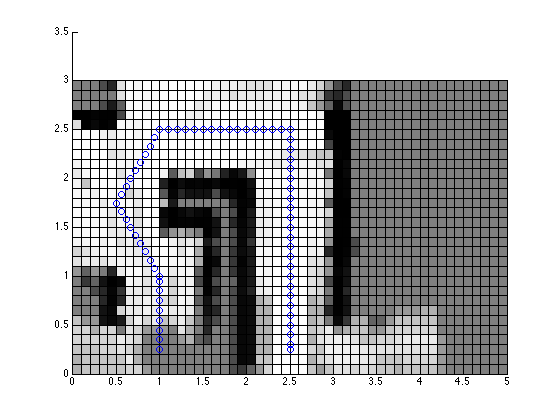
\includegraphics[scale=0.5]{Pictures/question3_100.png}
\caption{Map after 100 seconds}
\end{figure}

\begin{figure}[ht]
\hspace{0.5cm}
\centering
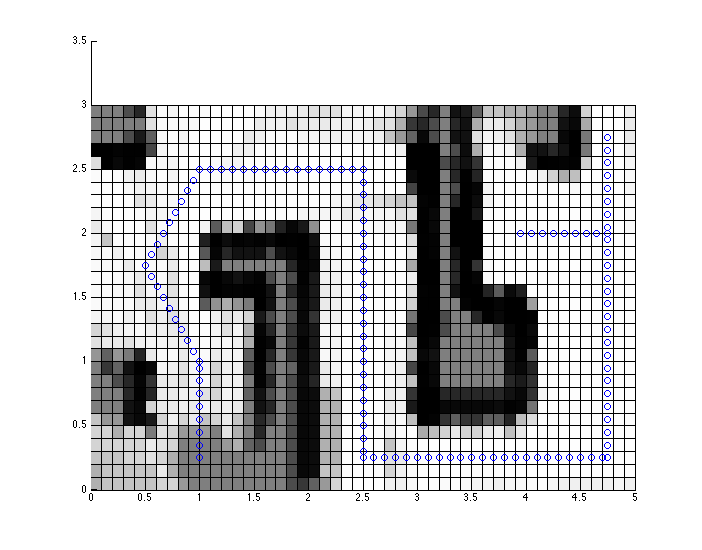
\includegraphics[scale=0.5]{Pictures/question3_200.png}
\caption{Map after 200 seconds}
\end{figure}

\newpage
\singlespacing
\section{Wavefront Exploration}
\setlength{\parindent}{1cm}

The modified wavefront algorithm used to dictate the robot's exploration pattern is based on the standard wavefront implementation provided to us in sample code. There are some minor changes. Within the wavefront algorithm, we consider a cell free if the probability that the cell is occupied is less than 0.6. We feed the wavefront algorithm the map that is being generated incrementally by the IR ranger inverse measurement model from the previous questions. The wavefront algorithm returns a path (in x and y coordinates) from the current starting point to the end point based on current knowledge of the map. This path is decided by assigning a cost to each cell on the map with lower costs being associated with shorter distances from the goal. The shortest path is then computed by stepping from the robot's position to the goal while always moving to cells of lower cost. More specifically, in this implementation each cell has a cost \textit{$c_i$} that is computed by checking the costs of its neighbouring cells and assigning a cost equal to 1 plus the lowest cost of any of the neighbouring cells. 
\begin{equation}
\onehalfspacing
\centering
\emph{$c_i$ = min($c_{neighbour_1}, c_{neighbour_2}, ... , c_{neighbour_n}$) + 1}
\end{equation}
In this case, we consider a neigbouring cell to be one that shares an edge (not just a vertex) with the cell in question. 

At every time step, we rescan and update probabilities in the map. Also at every time step we attempt to drive to the closest point in the path returned by the wavefront algorithm. When we reach the point, we make a new start position at our current position and run the wavepoint algorithm again. We then move to the closest point in the newly generated path and the cycle begins again. When the start point equals the end point, the robot has reached its goal. 

 \newpage
\singlespacing
\section{Wavefront Exploration Simulation}
\setlength{\parindent}{1cm}

\begin{figure}[ht]
\hspace{0.5cm}
\centering
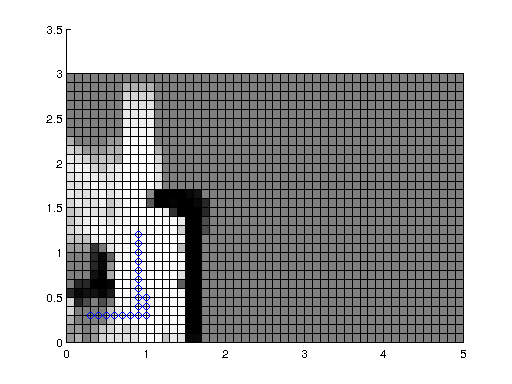
\includegraphics[scale=0.7]{Pictures/50_dt_scan.png}
\caption{Probability Map at Step 50}
\end{figure}

\begin{figure}[ht]
\hspace{0.5cm}
\centering
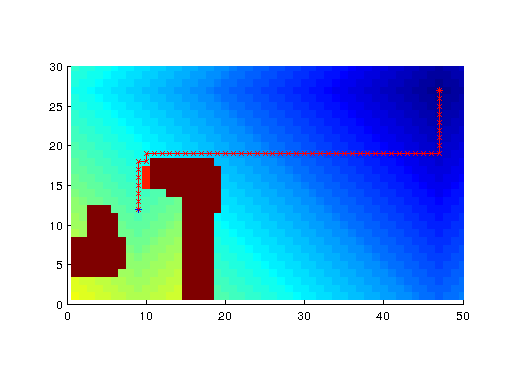
\includegraphics[scale=0.7]{Pictures/50_dt_wave.png}
\caption{Wavefront at Step 50}
\end{figure}

\begin{figure}[ht]
\hspace{0.5cm}
\centering
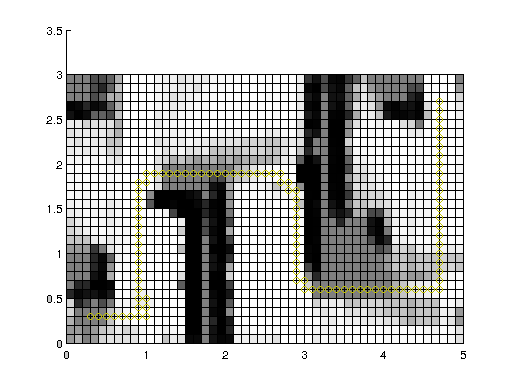
\includegraphics[scale=0.5]{Pictures/final_actual_scan.png}
\caption{Probability Map at Final Step}
\end{figure}

\begin{figure}[ht]
\hspace{0.5cm}
\centering
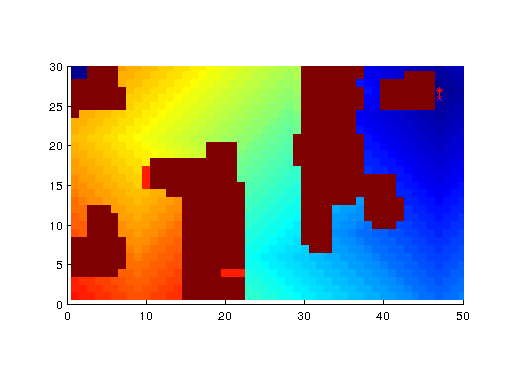
\includegraphics[scale=0.7]{Pictures/final_wave.png}
\caption{Wavefront at Final Step}
\end{figure}

To generate these plots we gave the wavefront scanner algoirthm starting and ending points of [0.3, 0.3] and [4.7, 2.7] respectively. Previously, we had chosen to pad the obstacles by 2 cells (20 cm) in order to prevent the robot from hitting the obstacles. However, with a padding of 2 cells, the endpoint was not in a viable location. Therefore, we made the assumption that the robot drives exactly in the centre of its current cell and reduced the padding to only 1 cell.  The blue and yellow circles on the probability maps show were the robot actually traveled. The obstacles you see in the wavefront figured have been dilated by 1 cell. In the wavefront figures you can see that the starting point for the wavefront path is being updated. At the final time step the starting point is about to equal the end point. 
 
 




\end{document}
